% This figure can be rendered by compiling the following LaTeX document:
%
% \documentclass[9pt, aspectratio=169]{beamer}
% \usetheme{metropolis}
% \usepackage{tikz}
% \usetikzlibrary{arrows.meta, positioning, backgrounds, fit}
% \begin{document}
% \begin{frame}[plain]
%     \begin{center}
%         \resizebox{0.8\textwidth}{!}{% This figure can be rendered by compiling the following LaTeX document:
%
% \documentclass[9pt, aspectratio=169]{beamer}
% \usetheme{metropolis}
% \usepackage{tikz}
% \usetikzlibrary{arrows.meta, positioning, backgrounds, fit}
% \begin{document}
% \begin{frame}[plain]
%     \begin{center}
%         \resizebox{0.8\textwidth}{!}{% This figure can be rendered by compiling the following LaTeX document:
%
% \documentclass[9pt, aspectratio=169]{beamer}
% \usetheme{metropolis}
% \usepackage{tikz}
% \usetikzlibrary{arrows.meta, positioning, backgrounds, fit}
% \begin{document}
% \begin{frame}[plain]
%     \begin{center}
%         \resizebox{0.8\textwidth}{!}{% This figure can be rendered by compiling the following LaTeX document:
%
% \documentclass[9pt, aspectratio=169]{beamer}
% \usetheme{metropolis}
% \usepackage{tikz}
% \usetikzlibrary{arrows.meta, positioning, backgrounds, fit}
% \begin{document}
% \begin{frame}[plain]
%     \begin{center}
%         \resizebox{0.8\textwidth}{!}{\input{synapse_2}}
%     \end{center}
% \end{frame}
% \end{document}


\begin{tikzpicture}[
    txt/.style={align=center},
    data/.style={-{Stealth[length=4pt]}, orange, dashed},
    ctrl/.style={-{Stealth[length=4pt]}, gray, dotted},
    api/.style={{Stealth[length=4pt]}-{Stealth[length=4pt]}, gray, dotted},
]

    \node[inner sep=0pt] (hpc) {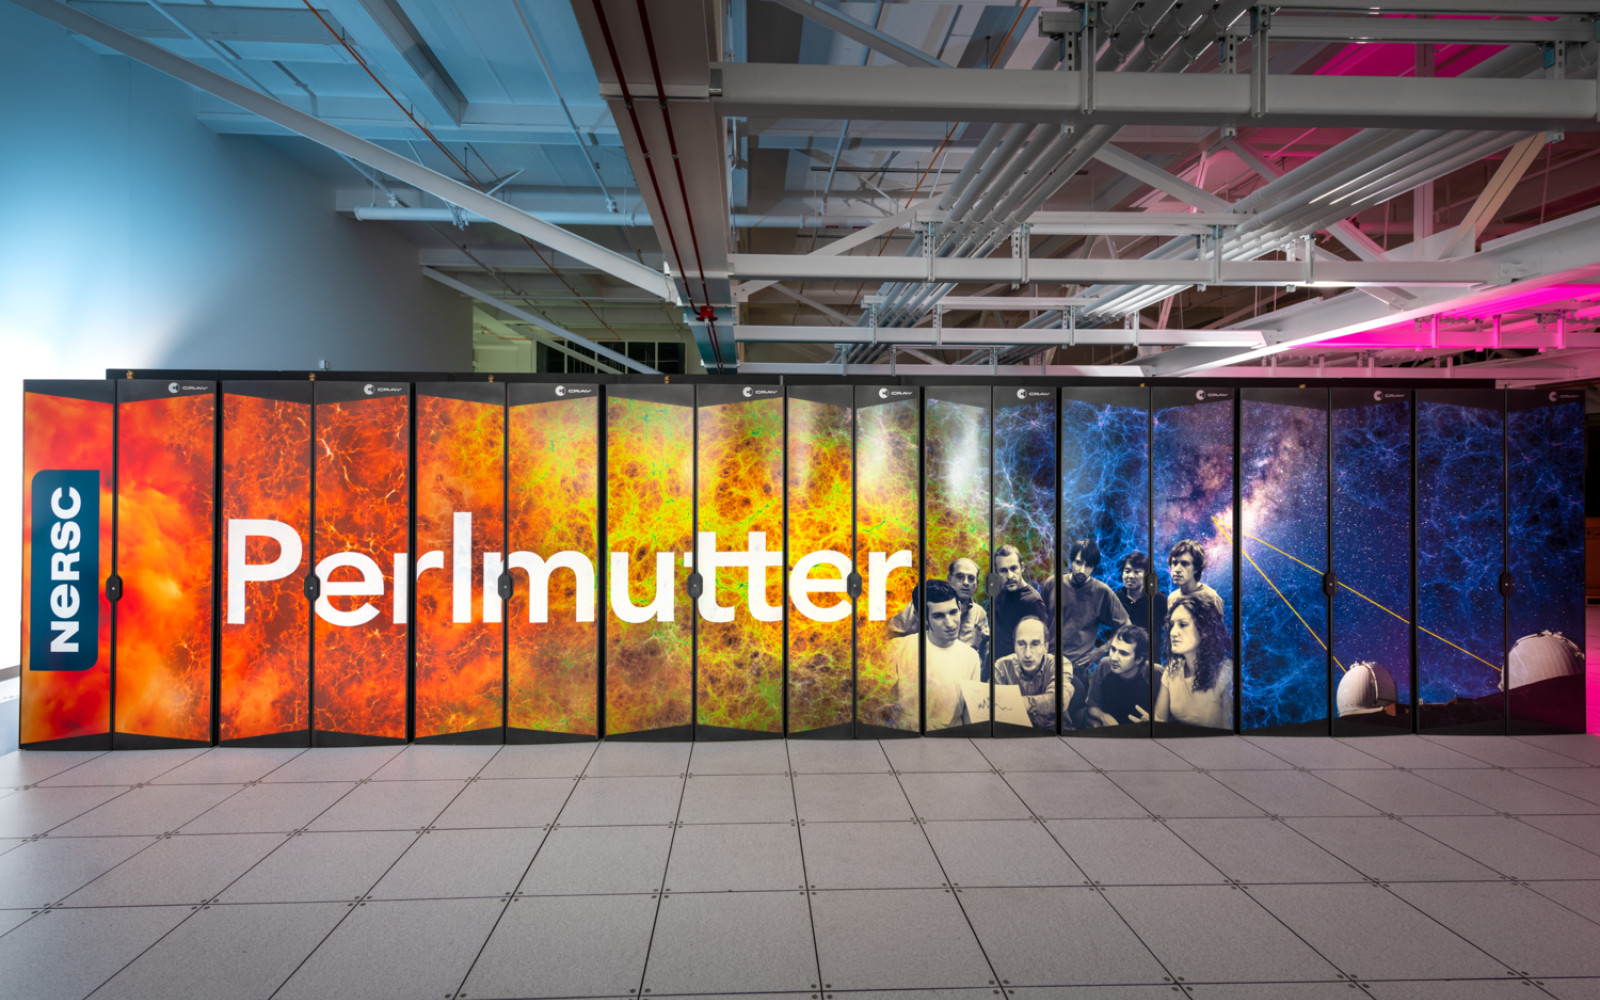
\includegraphics[width=2cm]{fig_perlmutter.jpg}};
    \node[txt, above=1pt of hpc] {Supercomputer};

    \node[inner sep=0pt, below=1.5cm of hpc] (exp) {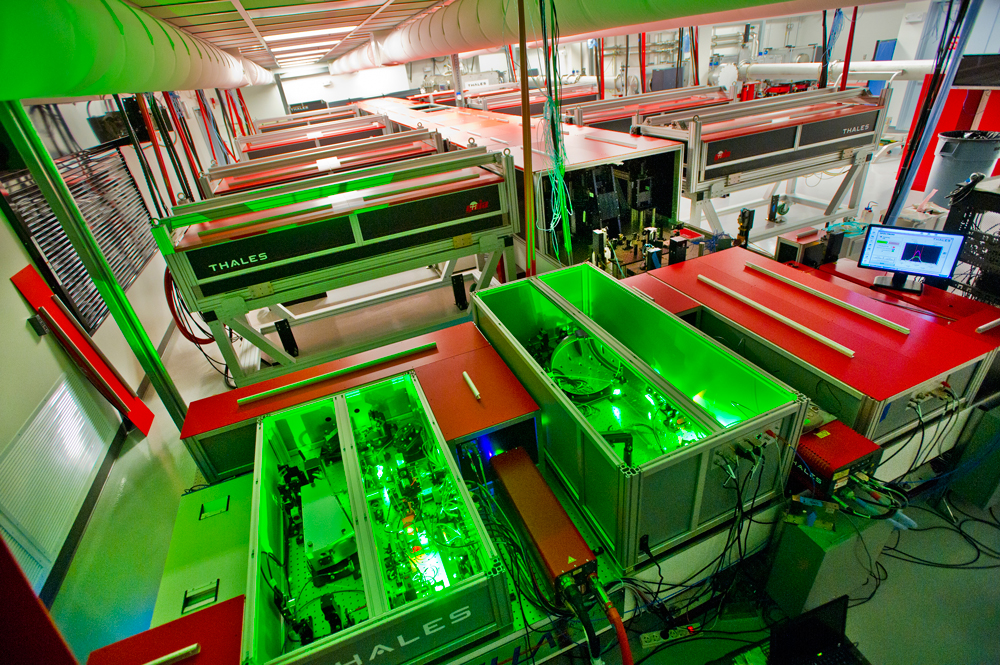
\includegraphics[width=2cm]{fig_bella.jpg}};
    \node[txt, below=1pt of exp] {Experiment};

    \node[inner sep=0pt, right=3.5cm of hpc, yshift=1.25cm] (ml) {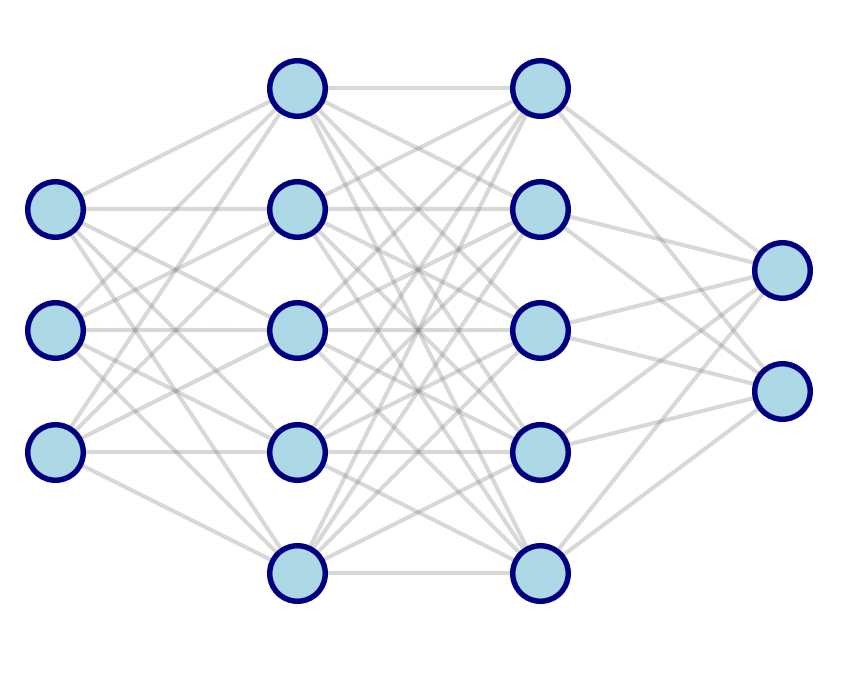
\includegraphics[width=2cm]{fig_ml.png}};
    \node[txt, above=1pt of ml] {AI/ML Models};

    \node[inner sep=0pt, right=3.5cm of hpc, yshift=-1.25cm] (db) {
\includegraphics[width=2cm]{fig_database.jpg}};
    \node[txt, below=1pt of db] {Database};

    \node[inner sep=0pt, right=8.5cm of hpc] (dashbe) {
\includegraphics[width=2cm]{fig_dashboard_backend.jpg}};
    \node[txt, above=1pt of dashbe] {Dashboard Backend};

    \node[inner sep=0pt, right=8.5cm of exp] (dashfe) {
\includegraphics[width=2cm]{fig_dashboard_frontend.jpg}};
    \node[txt, below=1pt of dashfe] {Dashboard Frontend};

    \draw[data] (exp) -- (db) node[midway, sloped, below] {write};
    \draw[data] (hpc) -- (db) node[midway, sloped, below] {read/write};
    \draw[data] (hpc) -- (ml) node[midway, sloped, below] {write};
    \draw[data] (dashbe) -- (db) node[midway, sloped, below] {read};
    \draw[data] (dashbe) -- (ml) node[midway, sloped, below] {read};
    \draw[ctrl] (dashbe) to[bend right=55] node[midway, above] {launch} (hpc);
    \draw[ctrl] (dashfe) to[bend right=-10] node[midway, below] {operator feedback} (exp);
    \draw[api] (dashfe) -- (dashbe);

\end{tikzpicture}}
%     \end{center}
% \end{frame}
% \end{document}


\begin{tikzpicture}[
    txt/.style={align=center},
    data/.style={-{Stealth[length=4pt]}, orange, dashed},
    ctrl/.style={-{Stealth[length=4pt]}, gray, dotted},
    api/.style={{Stealth[length=4pt]}-{Stealth[length=4pt]}, gray, dotted},
]

    \node[inner sep=0pt] (hpc) {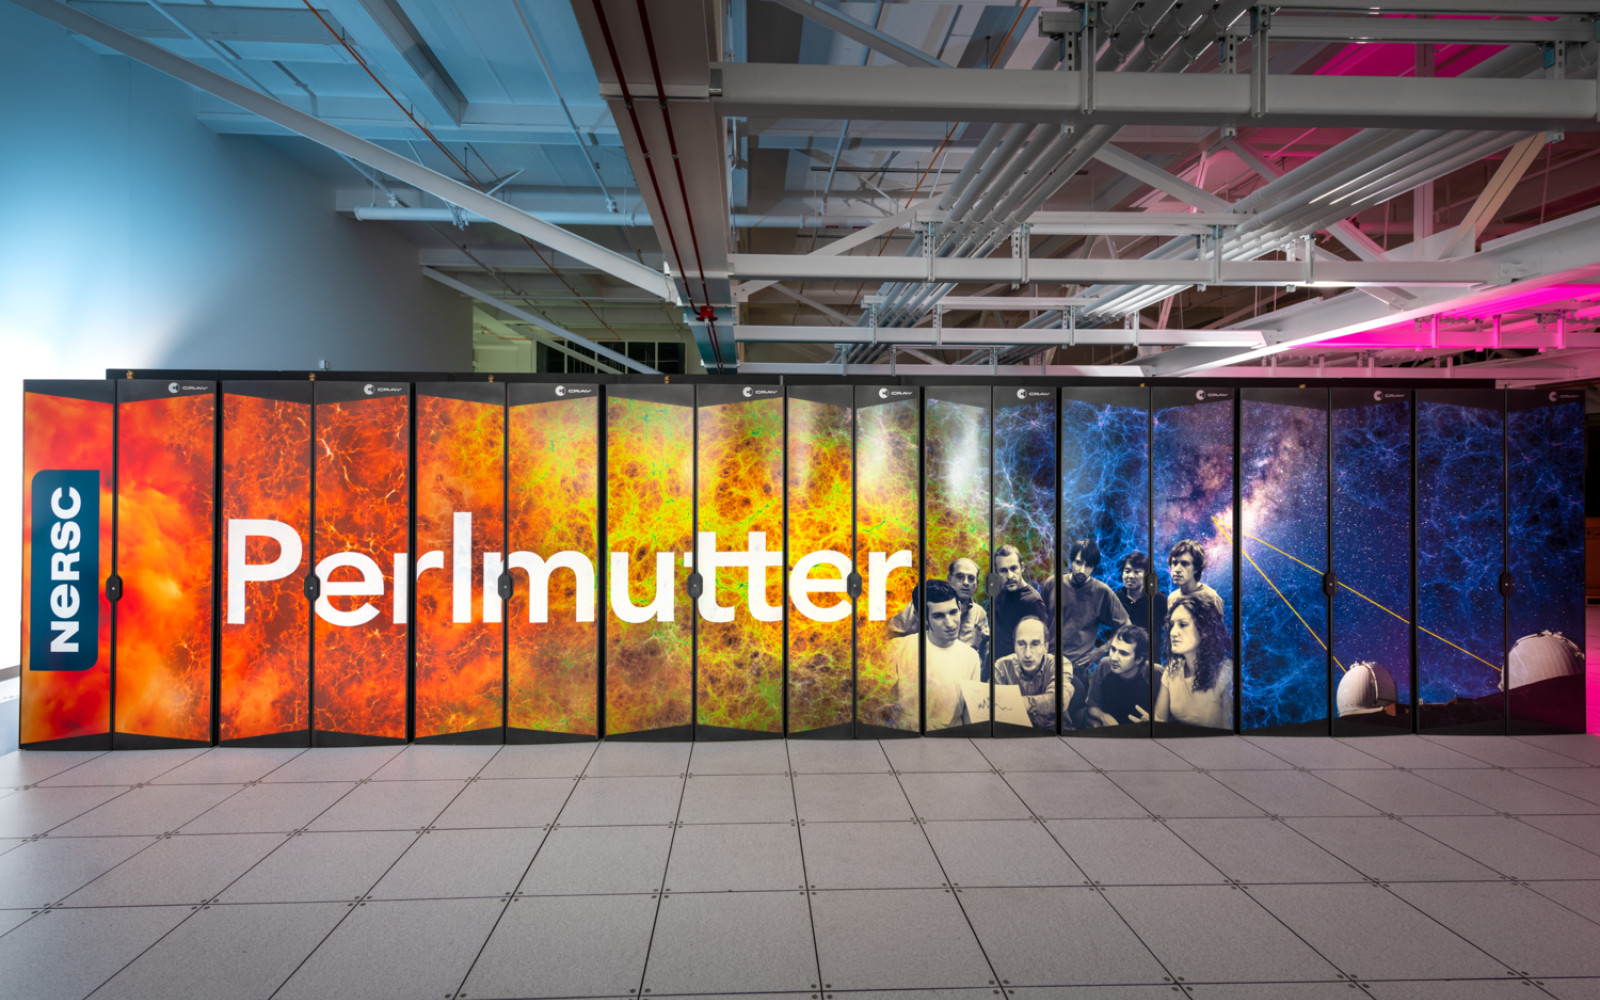
\includegraphics[width=2cm]{fig_perlmutter.jpg}};
    \node[txt, above=1pt of hpc] {Supercomputer};

    \node[inner sep=0pt, below=1.5cm of hpc] (exp) {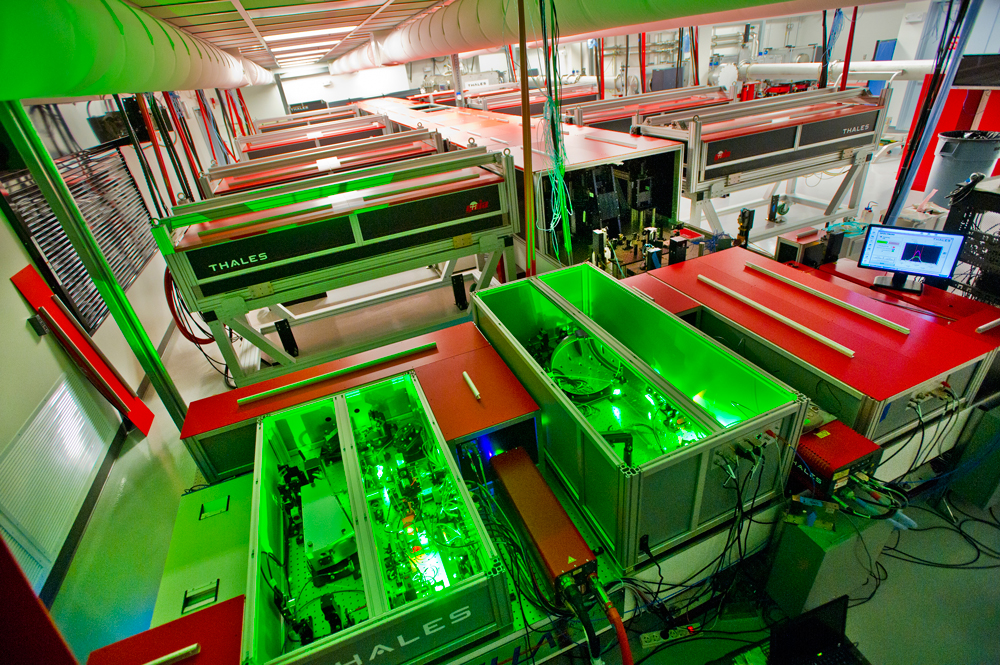
\includegraphics[width=2cm]{fig_bella.jpg}};
    \node[txt, below=1pt of exp] {Experiment};

    \node[inner sep=0pt, right=3.5cm of hpc, yshift=1.25cm] (ml) {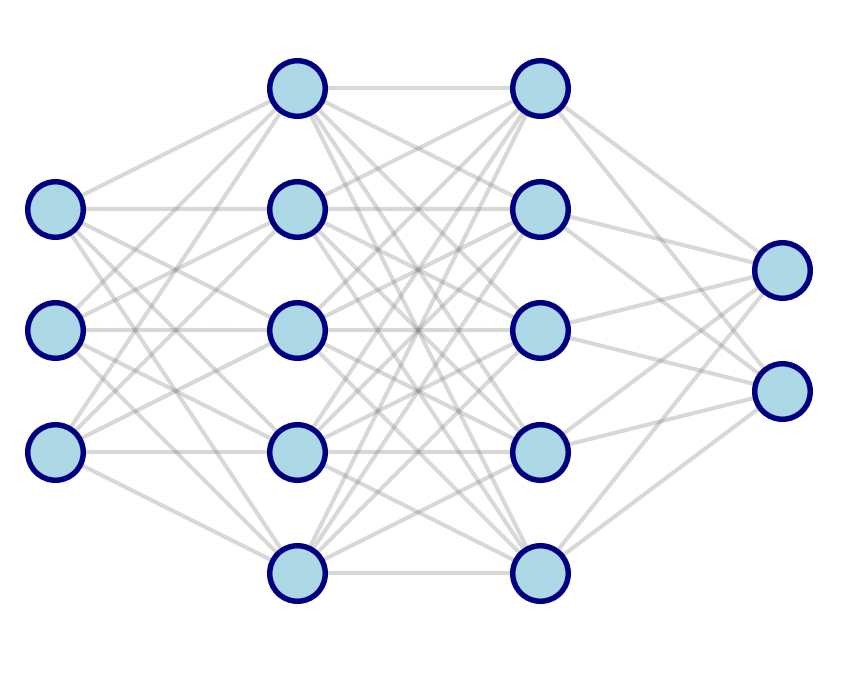
\includegraphics[width=2cm]{fig_ml.png}};
    \node[txt, above=1pt of ml] {AI/ML Models};

    \node[inner sep=0pt, right=3.5cm of hpc, yshift=-1.25cm] (db) {
\includegraphics[width=2cm]{fig_database.jpg}};
    \node[txt, below=1pt of db] {Database};

    \node[inner sep=0pt, right=8.5cm of hpc] (dashbe) {
\includegraphics[width=2cm]{fig_dashboard_backend.jpg}};
    \node[txt, above=1pt of dashbe] {Dashboard Backend};

    \node[inner sep=0pt, right=8.5cm of exp] (dashfe) {
\includegraphics[width=2cm]{fig_dashboard_frontend.jpg}};
    \node[txt, below=1pt of dashfe] {Dashboard Frontend};

    \draw[data] (exp) -- (db) node[midway, sloped, below] {write};
    \draw[data] (hpc) -- (db) node[midway, sloped, below] {read/write};
    \draw[data] (hpc) -- (ml) node[midway, sloped, below] {write};
    \draw[data] (dashbe) -- (db) node[midway, sloped, below] {read};
    \draw[data] (dashbe) -- (ml) node[midway, sloped, below] {read};
    \draw[ctrl] (dashbe) to[bend right=55] node[midway, above] {launch} (hpc);
    \draw[ctrl] (dashfe) to[bend right=-10] node[midway, below] {operator feedback} (exp);
    \draw[api] (dashfe) -- (dashbe);

\end{tikzpicture}}
%     \end{center}
% \end{frame}
% \end{document}


\begin{tikzpicture}[
    txt/.style={align=center},
    data/.style={-{Stealth[length=4pt]}, orange, dashed},
    ctrl/.style={-{Stealth[length=4pt]}, gray, dotted},
    api/.style={{Stealth[length=4pt]}-{Stealth[length=4pt]}, gray, dotted},
]

    \node[inner sep=0pt] (hpc) {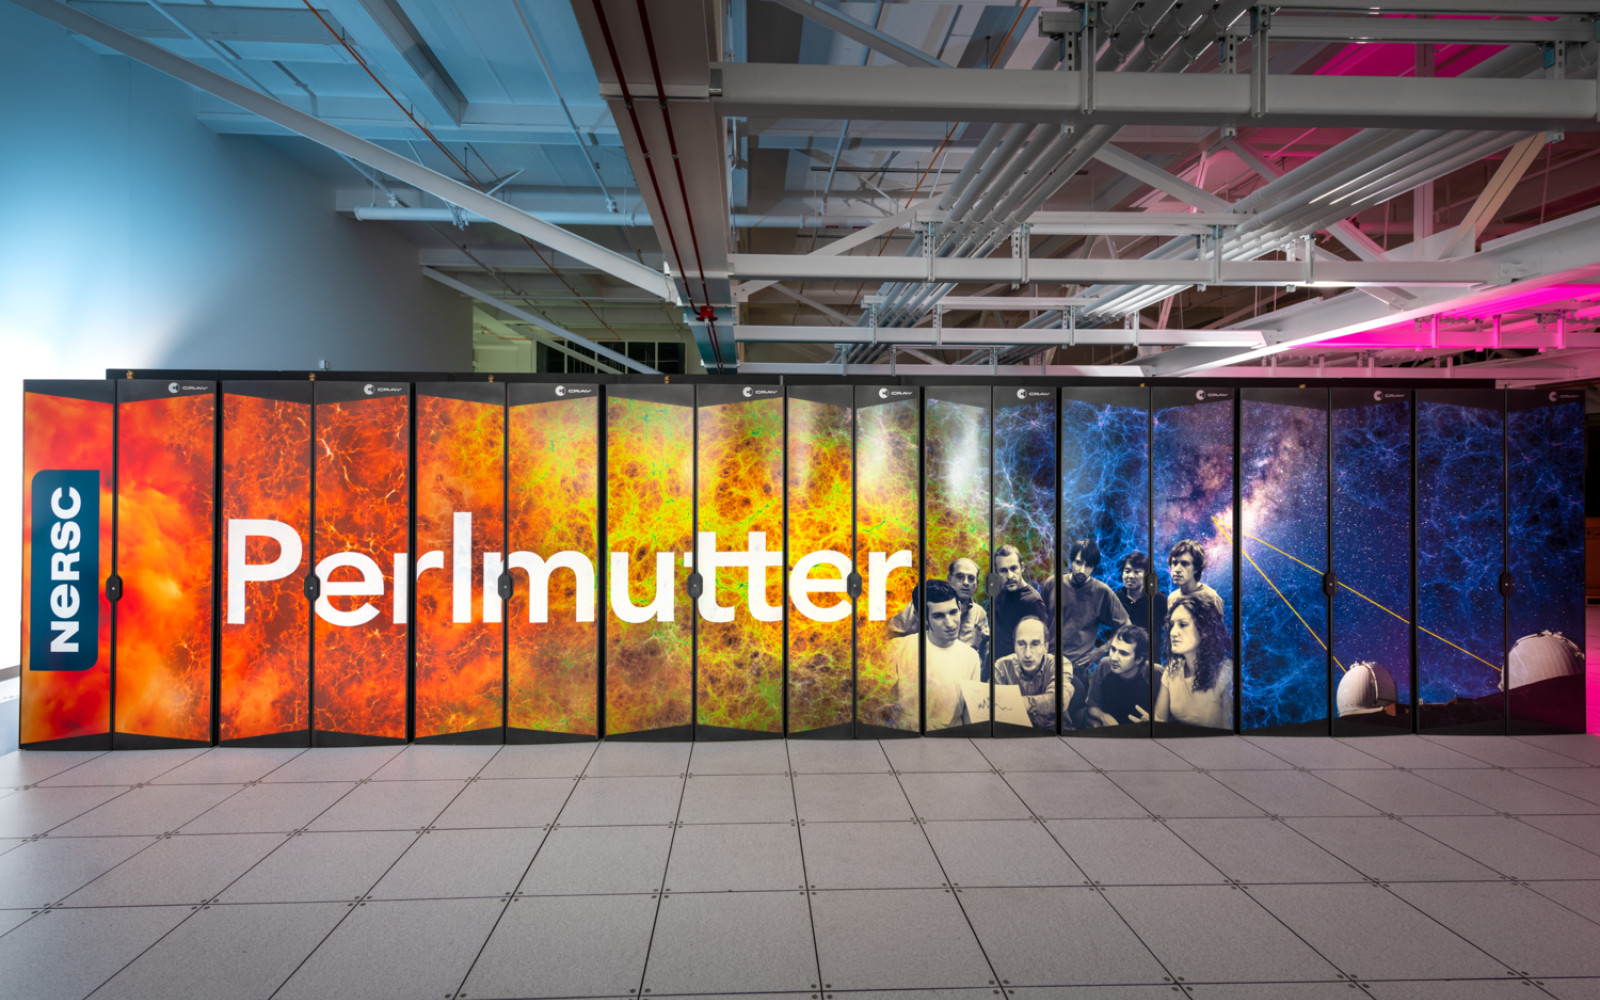
\includegraphics[width=2cm]{fig_perlmutter.jpg}};
    \node[txt, above=1pt of hpc] {Supercomputer};

    \node[inner sep=0pt, below=1.5cm of hpc] (exp) {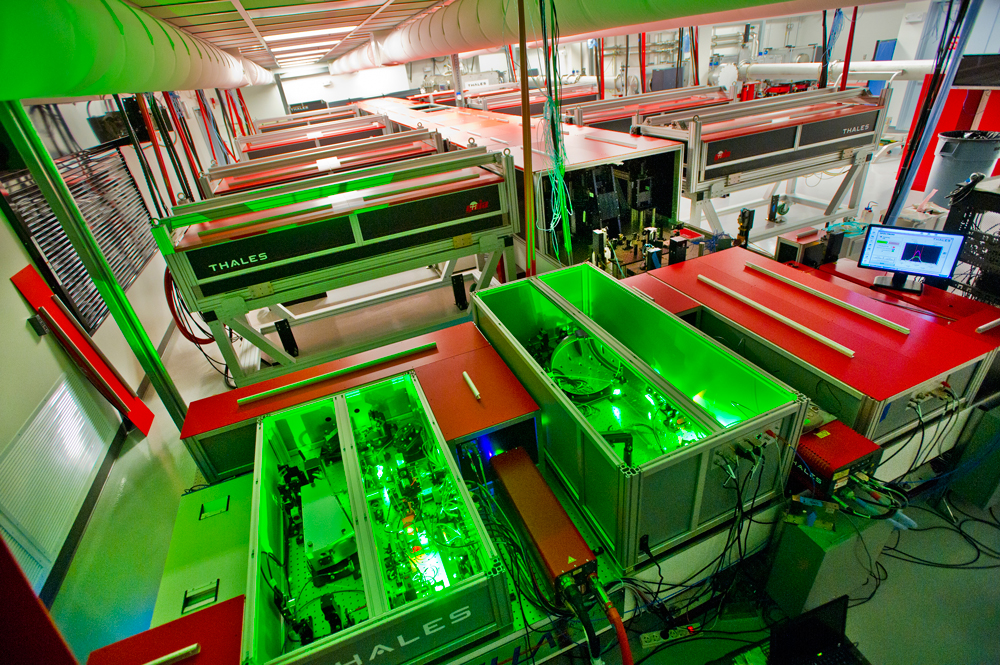
\includegraphics[width=2cm]{fig_bella.jpg}};
    \node[txt, below=1pt of exp] {Experiment};

    \node[inner sep=0pt, right=3.5cm of hpc, yshift=1.25cm] (ml) {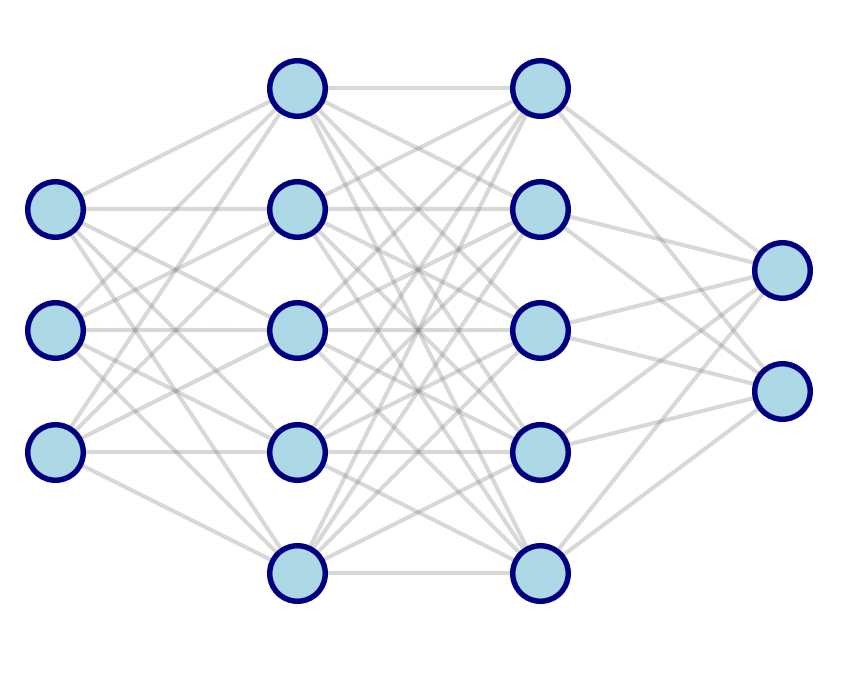
\includegraphics[width=2cm]{fig_ml.png}};
    \node[txt, above=1pt of ml] {AI/ML Models};

    \node[inner sep=0pt, right=3.5cm of hpc, yshift=-1.25cm] (db) {
\includegraphics[width=2cm]{fig_database.jpg}};
    \node[txt, below=1pt of db] {Database};

    \node[inner sep=0pt, right=8.5cm of hpc] (dashbe) {
\includegraphics[width=2cm]{fig_dashboard_backend.jpg}};
    \node[txt, above=1pt of dashbe] {Dashboard Backend};

    \node[inner sep=0pt, right=8.5cm of exp] (dashfe) {
\includegraphics[width=2cm]{fig_dashboard_frontend.jpg}};
    \node[txt, below=1pt of dashfe] {Dashboard Frontend};

    \draw[data] (exp) -- (db) node[midway, sloped, below] {write};
    \draw[data] (hpc) -- (db) node[midway, sloped, below] {read/write};
    \draw[data] (hpc) -- (ml) node[midway, sloped, below] {write};
    \draw[data] (dashbe) -- (db) node[midway, sloped, below] {read};
    \draw[data] (dashbe) -- (ml) node[midway, sloped, below] {read};
    \draw[ctrl] (dashbe) to[bend right=55] node[midway, above] {launch} (hpc);
    \draw[ctrl] (dashfe) to[bend right=-10] node[midway, below] {operator feedback} (exp);
    \draw[api] (dashfe) -- (dashbe);

\end{tikzpicture}}
%     \end{center}
% \end{frame}
% \end{document}


\begin{tikzpicture}[
    txt/.style={align=center},
    data/.style={-{Stealth[length=4pt]}, orange, dashed},
    ctrl/.style={-{Stealth[length=4pt]}, gray, dotted},
    api/.style={{Stealth[length=4pt]}-{Stealth[length=4pt]}, gray, dotted},
]

    \node[inner sep=0pt] (hpc) {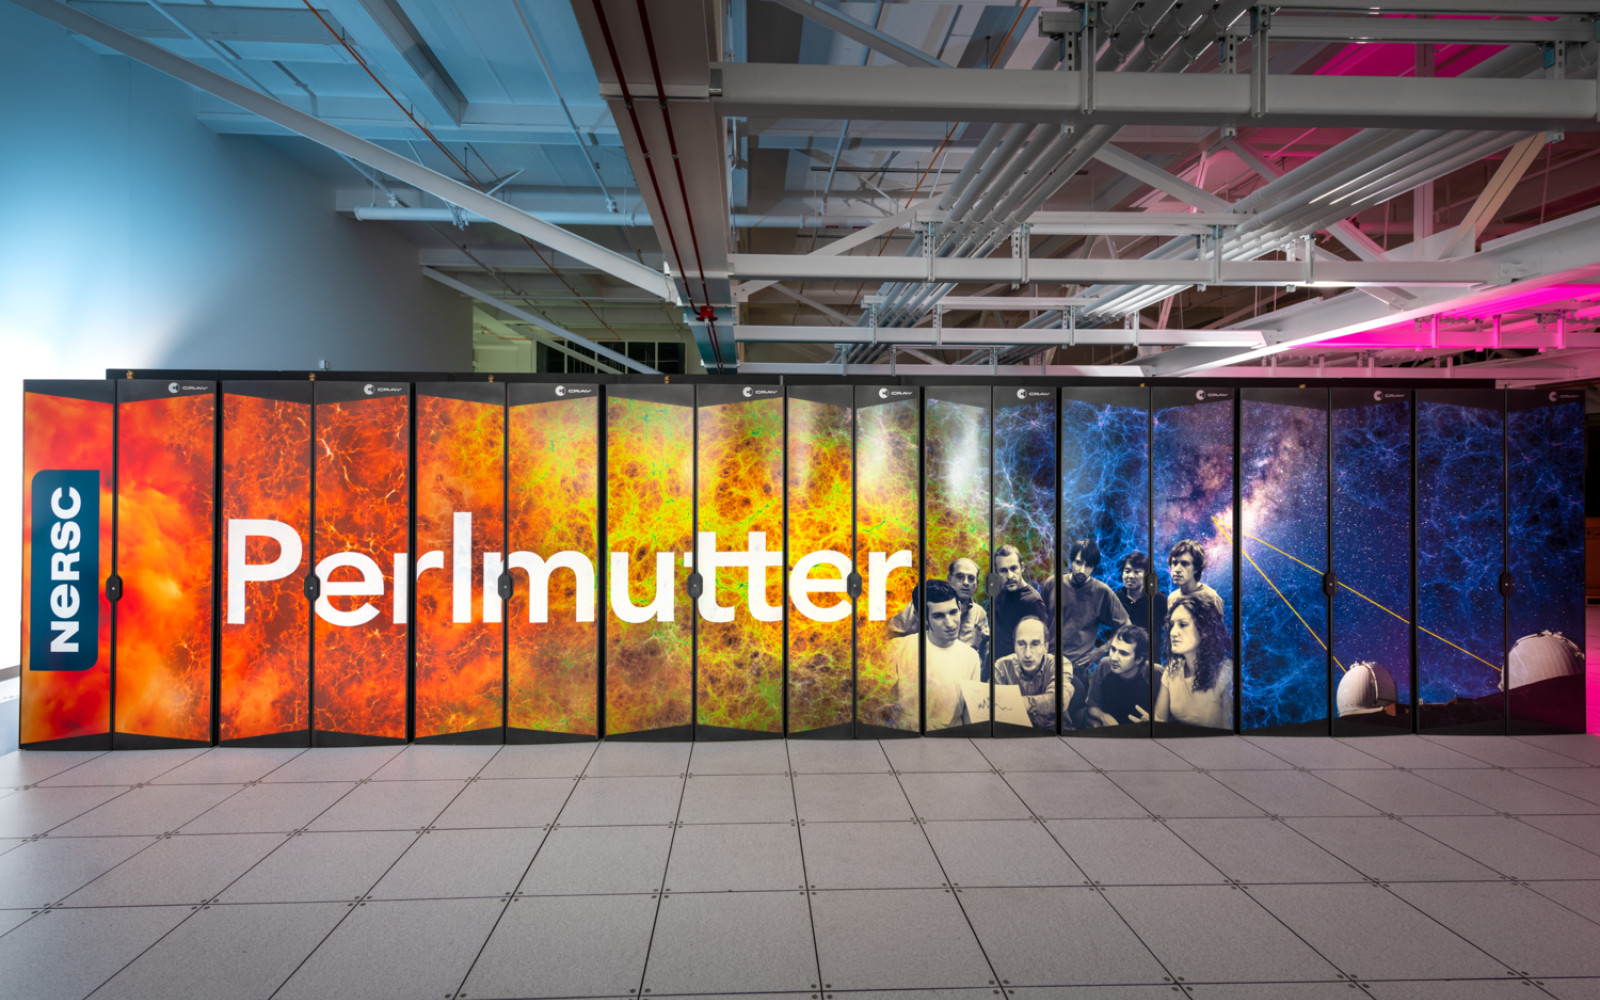
\includegraphics[width=2cm]{fig_perlmutter.jpg}};
    \node[txt, above=1pt of hpc] {Supercomputer};

    \node[inner sep=0pt, below=1.5cm of hpc] (exp) {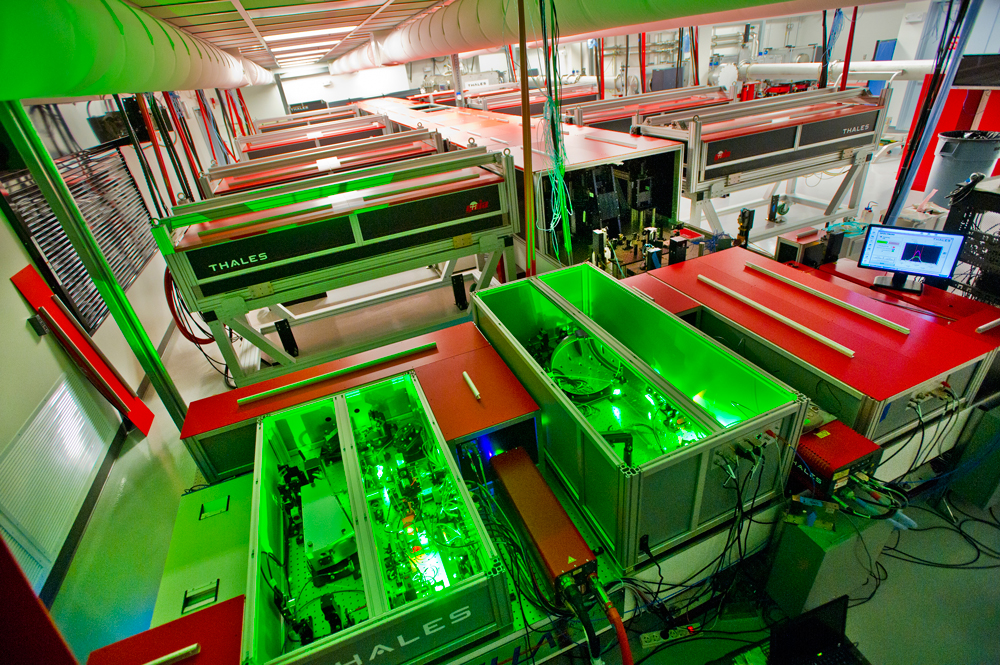
\includegraphics[width=2cm]{fig_bella.jpg}};
    \node[txt, below=1pt of exp] {Experiment};

    \node[inner sep=0pt, right=3.5cm of hpc, yshift=1.25cm] (ml) {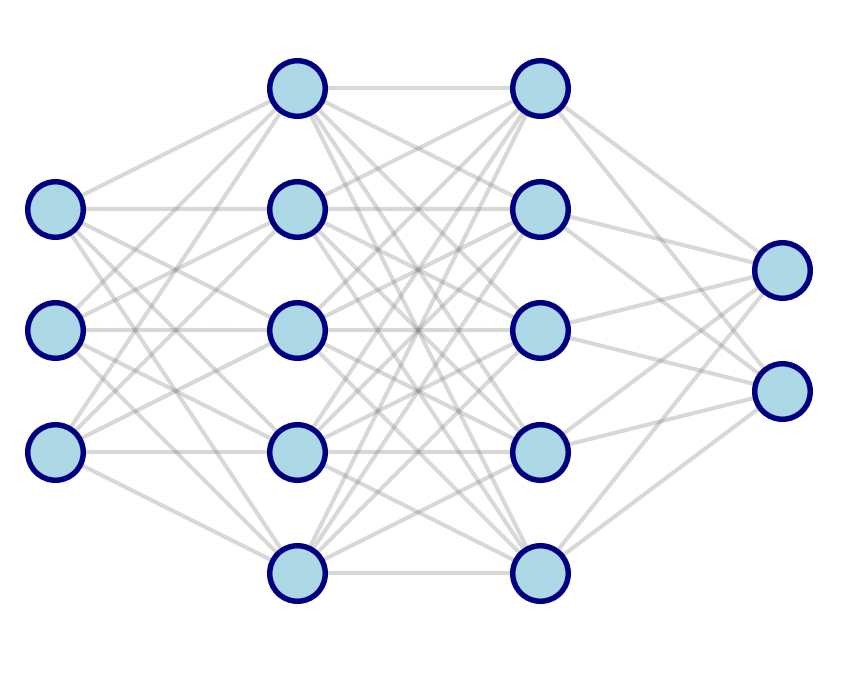
\includegraphics[width=2cm]{fig_ml.png}};
    \node[txt, above=1pt of ml] {AI/ML Models};

    \node[inner sep=0pt, right=3.5cm of hpc, yshift=-1.25cm] (db) {
\includegraphics[width=2cm]{fig_database.jpg}};
    \node[txt, below=1pt of db] {Database};

    \node[inner sep=0pt, right=8.5cm of hpc] (dashbe) {
\includegraphics[width=2cm]{fig_dashboard_backend.jpg}};
    \node[txt, above=1pt of dashbe] {Dashboard Backend};

    \node[inner sep=0pt, right=8.5cm of exp] (dashfe) {
\includegraphics[width=2cm]{fig_dashboard_frontend.jpg}};
    \node[txt, below=1pt of dashfe] {Dashboard Frontend};

    \draw[data] (exp) -- (db) node[midway, sloped, below] {write};
    \draw[data] (hpc) -- (db) node[midway, sloped, below] {read/write};
    \draw[data] (hpc) -- (ml) node[midway, sloped, below] {write};
    \draw[data] (dashbe) -- (db) node[midway, sloped, below] {read};
    \draw[data] (dashbe) -- (ml) node[midway, sloped, below] {read};
    \draw[ctrl] (dashbe) to[bend right=55] node[midway, above] {launch} (hpc);
    \draw[ctrl] (dashfe) to[bend right=-10] node[midway, below] {operator feedback} (exp);
    \draw[api] (dashfe) -- (dashbe);

\end{tikzpicture}